\section{Theoretical Background} \label{sec:theory}
The purpose of this chapter is to go through the basic wind turbine theory. 

\subsection{Aerodynamics}
The sun delivers energy to the earth by heating up the surface and subsequently the air of the earth. Winds occur as a result of the pressure differences that occur due to the expansion and contraction of the air. \\

Wind turbines work because they are able to convert the wind's energy into a torque in the generator which then generates electrical energy. When the wind blows over the blades of a wind turbine it delivers some of its energy to the blade, yielding both a thrust force and torque. The delivery of energy results in a lowing of the wind speed and due to mass retention, an expansion, immediately following the rotor area as seen in \cref{fig:betz}.
\begin{figure}[h]
	\centering
	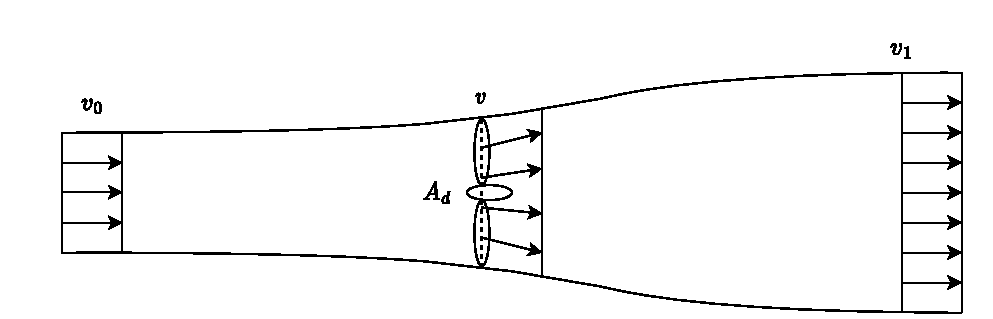
\includegraphics[width=0.8\linewidth]{Graphics/FlowThroughRotor.pdf}
	\caption{This is a caption}
	\label{fig:betz}
\end{figure}

The energy in the wind can be expressed as kinetic energy:
\begin{equation} \label{eq:energy}
	E = \dfrac{1}{2} m v^2
\end{equation}
Subsequently the power can be calculated as the time derivative of the energy:
\begin{equation} \label{eq:power}
	P = \dot{E} = \dfrac{1}{2} \dot{m} v^2
\end{equation}
The time derivative of the mass can be expressed from the air density $ \rho $, the cross-sectional area $ A_d $and the wind velocity $ v $:
\begin{equation}\label{eq:mass_deriv}
	\dot{m} = \rho A_d v
\end{equation}
Combining \cref{eq:mass_deriv} and \cref{eq:mass_deriv} yields:
\begin{equation}\label{eq:power2}
	P_{air} = \dfrac{1}{2} \rho A_d v^3
\end{equation}
The percentage of the available power that it is possible to extract from the wind is expressed with the performance coefficient $ C_p $ as such:
\begin{equation}\label{eq:power_w_Cp}
	P_{T} = \dfrac{1}{2} \rho A_d v^3 C_p
\end{equation}